
\chapter{Results}
The culminating part of this nuclear physics analysis begins with the extraction of the experimentally measured DIS cross sections for three targets. Then using those cross sections to study the per nucleon scaled A/D ratio. I will also use these A/D ratios to study the EMC effect for both helium-3 and tritium. In this chapter, I will present my results for the DIS cross sections and EMC effect. I will also discuss an error analysis for both the cross section measurements and the EMC effect results. 
\section{DIS Cross Section}
\paragraph{}Using the Monte Carlo ratio method, I extracted the experimental measured cross section for helium-3, tritium, and deuterium. These DIS cross section extraction ranges from 0.18 to 0.82 in $x$, from 2.2 to 11.8 GeV$^2$ in $Q^2$, and has W$^2$ $>3.5$ GeV$^2$. The central momentum setting of the spectrometer is 3.1 GeV/c and the spectrometer was moved from 17.5 to 33.5 degrees.
\begin{figure}
	\caption{The ratio of data to Monte Carlo yield in bins of $x$. The top plot is on kinematic basis. The bottom plot uses good electron count weighting technique discusses in section \ref{sec:Yield} to combine the overlapping kinematics.\label{D_MC_COMP}}
	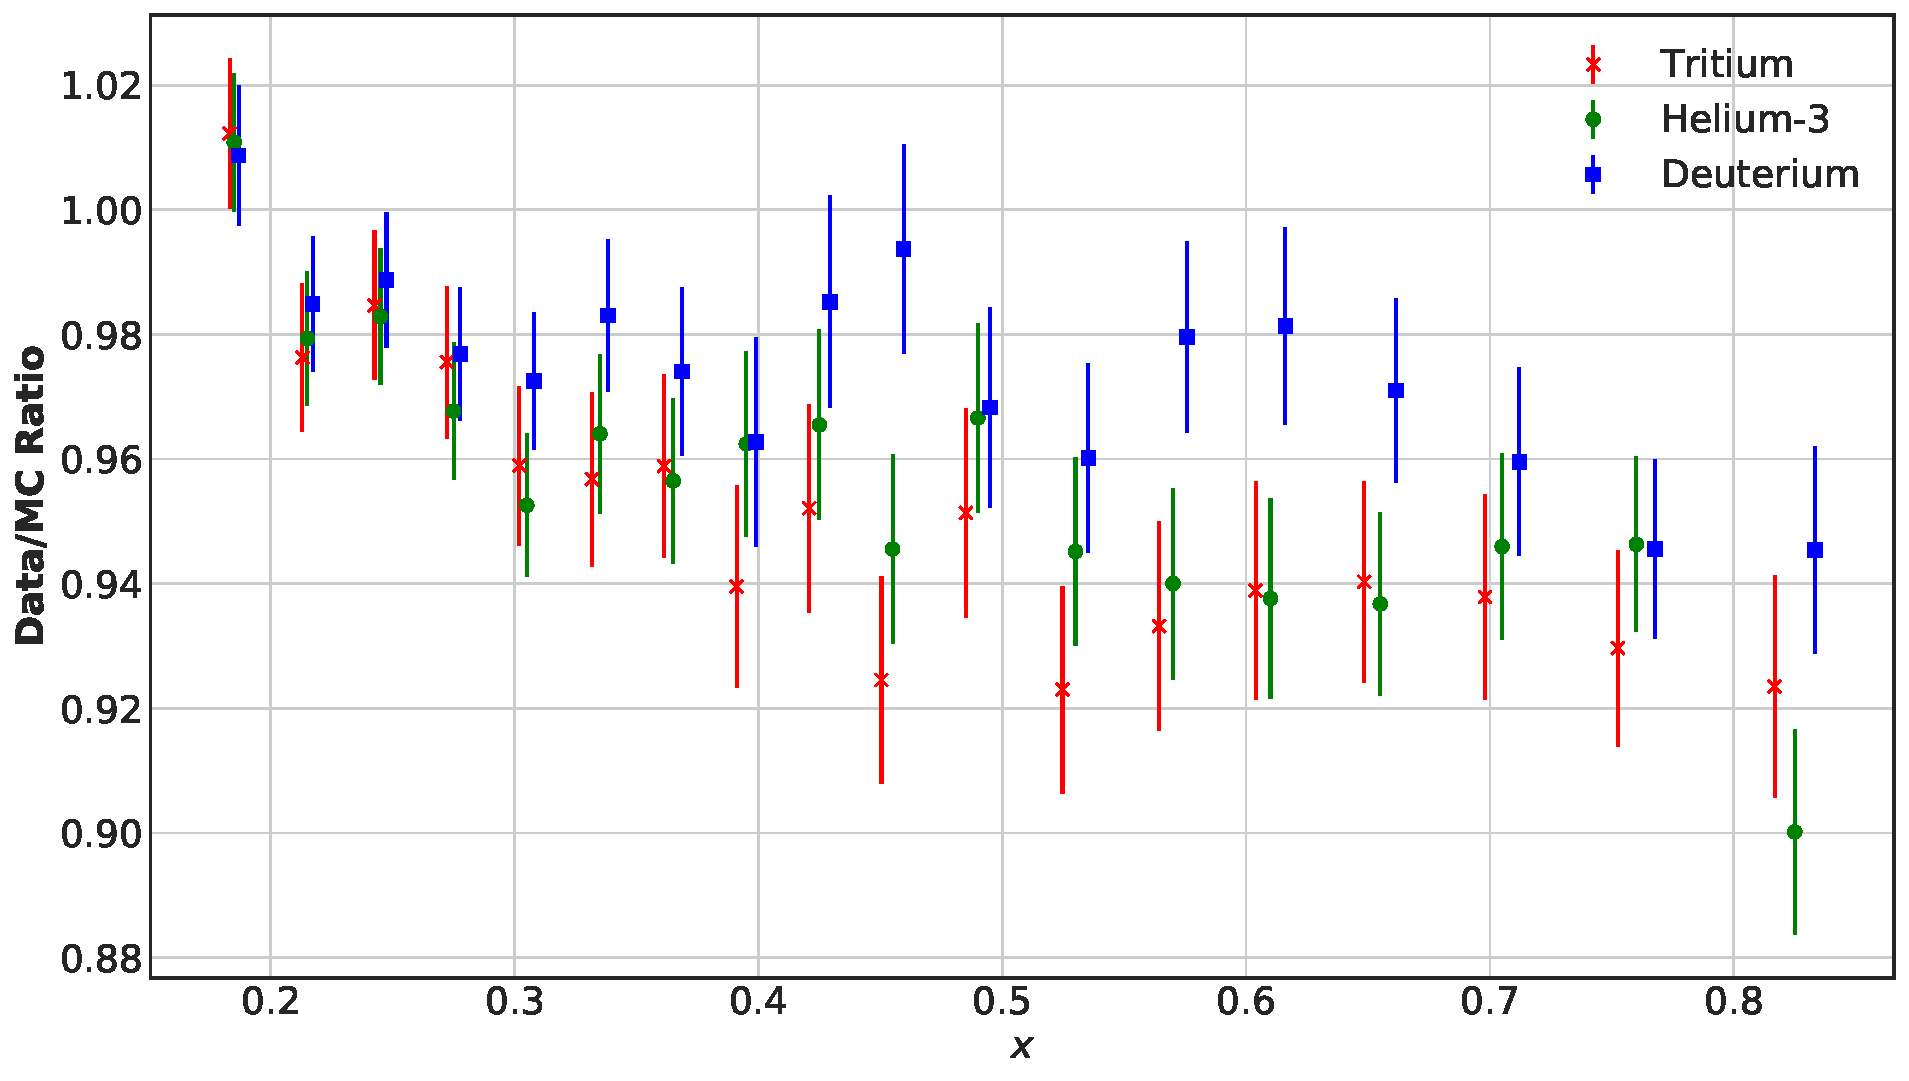
\includegraphics[width=15cm]{Ratio_all.pdf}
\end{figure}
\begin{equation}
\sigma_{Data} = \sigma_{model} \cdot \frac{Y_{Data}}{Y_{MC}}. \nonumber
\end{equation} 

I compared the data yield to the Monte Carlo yield to produce a correcting factor for the model cross section. Figure \ref{D_MC_COMP} shows the ratio comparison between data and Monte Carlo in bins of $x$ for each kinematic measurement and the combined ratio for the overlapping bins. Then apply the ratio factor for a bin in $x$ to the model cross section to extract out the experimentally measured cross section for that bin. Figure \ref{CCplot} show a plot of the experientially measured cross section for tritium, helium-3, and deuterium. This measurement includes a total normalization uncertainty due to the target thickness measurement uncertainty, tritium= 0.97\%, helium-3 = 1.12\%, and deuterium = 0.56\% \cite{HATT_eng}. The measurement uncertainties for each gas target are displayed in table \ref{tgt_table}. 

\begin{figure}
	\hspace{-80pt}
	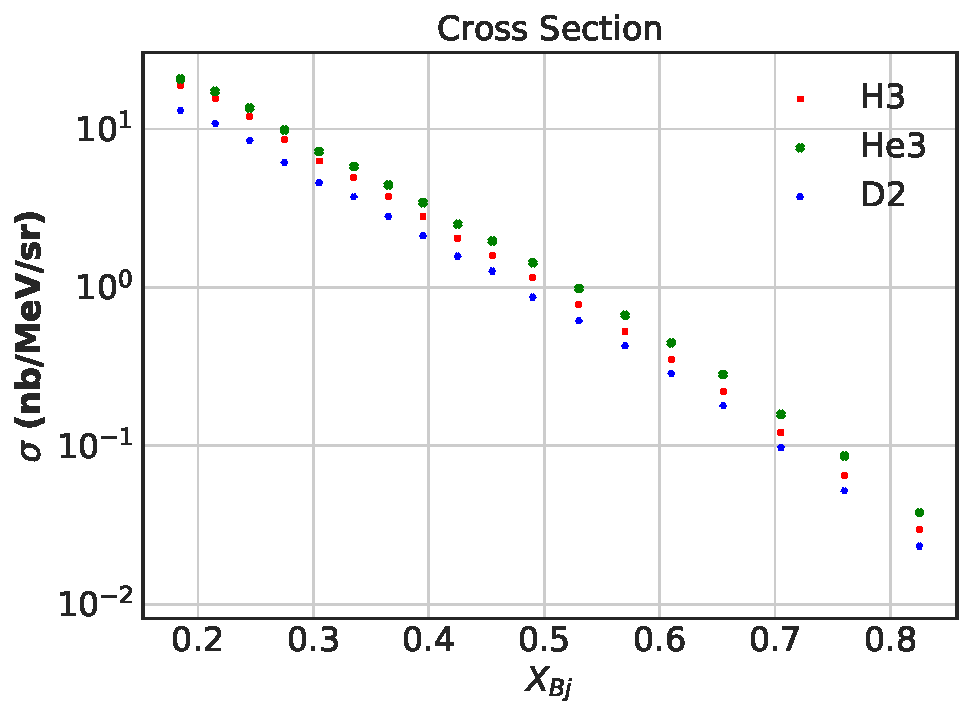
\includegraphics[width=19cm]{total_xs.pdf}
	\caption{Experimentally measured cross section using the Monte Carlo ratio method for tritium, helium-3, and deuterium. Normalization uncertainty due to target thickness uncertainty for tritium= 0.97\%, helium-3 = 1.12\%, and deuterium = 0.56\%. \label{CCplot}}
\end{figure}

\section{Cross Section Error Analysis}
The measurement of the cross section requires finally tune detectors and analysis process. Uncertainties arise due to the nature and limitations of these spectrometers and the analysis of the data received. In this section, I will discuss the calculation and propagation of errors in the analysis of the DIS cross section. The error analysis will be broken into the calculation of normalized yield for data, yield for Monte Carlo, and the cross section extraction. 
\begin{align}
\dfrac{d\sigma}{dE^{\prime}d\Omega} &= \frac{(N - BG)}{\mathscr{L} \cdot \epsilon \cdot \Delta E^{\prime} \Delta \Omega \cdot A(E^{\prime},\theta)}. \nonumber\\
\sigma &= \text{NormY}/\left(\Delta E^{\prime} \Delta \Omega \cdot A(E^{\prime},\theta)\right)\nonumber\\
\text{NormY} &= \left(N_e \cdot BG/\epsilon \right) / \mathscr{L}
\end{align}
\paragraph{}
The contributions for error on the measurement of the normalized yield(normY) can be simplified into the contributions for the corrected number of electrons and the luminosity. The error for the corrected number of counted electrons includes the random statistical error for the count of electrons detected, the error associated with the calculated efficiencies, and the error from the background correction. The electron statics range from 4875 to more then 42000 in a bin and therefor I have treated the randomness of the counting in a standard error technique. The relative statistical error for a bin is $\frac{1}{\sqrt{Ne}}$ and ranges from 1.4\% to 0.5\%. Calculating the efficiencies deals with calculating a probability of a binomial choice. The errors associated with the efficiencies are calculated using the Wilson score interval described in equation \ref{WSI}, where $p$ is the efficiency or a probability of a success, $n$ is the number of samples, $z$ is 1.645 for a 95\% confidence level. The individual efficiency errors are added in quadrature to calculate an over all efficiency error.
\begin{equation}
p[_{UpperBound},_{LowerBound}] = \frac{ 2np +z^2 \pm \left[z\sqrt{z^2 - \frac{1}{n} + 4np(1-p) +(4p-2)} + 1 \right]}{2(n+z^2)} \label{WSI}
\end{equation}


Measurements of the target thicknesses uncertainty are associated with an overall normalization uncertainty that could cause the value of the cross section for all bins to increase or decrease uniformly.


\begin{table}[]
	\caption{Relative Error Contributions in $\%$ for Cross Section for a selection of bins. The efficiency error is a combination of the error from the livetime, PID, tracking, and trigger efficiency calculations.}
	\centering
	\begin{tabular}{|l|l|l|l|}
		\hline
		\textbf{\qquad \qquad\qquad x bin}   & \textbf{0.215} & \textbf{0.455} & \textbf{0.705} \\ \hline\hline
		Statistical             & 0.512 & 0.889 & 1.106 \\ \hline
		Efficiency Error*       & 0.665 & 1.477 & 2.951 \\ \hline
		??Optics 				& ?0.665& ?1.477 &?2.951 \\ \hline
		Positron Correction     & 0.036 & 0.016 & 0.005 \\ \hline
		Density Correction      & 0.002 & 0.002 & 0.002 \\ \hline
		Monte Carlo Statistical & 0.193 & 0.217 & 0.209 \\ \hline
		??Cross Section Model 	& ?0.193 & ?0.217 & ?0.209 \\ \hline
		??Radiative Corrections\cite{primer} 	& 0.5  & 0.5 & 0.5 \\ \hline
		Total Error		 	 	& 0.95  & 1.931 & 3.316 \\ \hline
	\end{tabular}
\end{table}
\cite{Ar_Ti}


\section{EMC Ratios}

\subsection{Isoscalar Correction}
\subsection{EMC Effect}

